\documentclass[dvisvgm]{standalone}

\usepackage{tikz}
\usepackage{fontawesome5}

\usetikzlibrary{%
    arrows,
    arrows.meta,
    decorations,
    backgrounds,
    positioning,
    fit,
    graphs,
    petri,
    shadows,
    datavisualization.formats.functions,
    calc,
    shapes,
    shapes.multipart,
    matrix,
    plotmarks
}

\begin{document}
\begin{tikzpicture}[]
    \node[draw, fill=blue!5, minimum height=4cm, minimum width=16cm] (cluster) {};

    \matrix[column sep=1cm, row sep=1cm] at (cluster.center) {
        &\node[draw, fill=white] (ss1)  {\faIcon{database} StatefulSet 1};
        &\node[draw, fill=white] (ss2) {\faIcon{database} StatefulSet 2};
        &\node {\dots};
        &\node[draw, fill=white] (ssn) {\faIcon{database} StatefulSet N};
        \\

        \node[draw, fill=white] (openvpn) {\faIcon{user-secret} OpenVPN};
        &\node[draw, fill=white] (s1) {\faIcon{network-wired} Service 1};
        &\node[draw, fill=white] (s2) {\faIcon{network-wired} Service 2};
        &\node {\dots};
        &\node[draw, fill=white] (sn) {\faIcon{network-wired} Service N};
        \\
    };

    \node[draw, fill=gray!10, minimum height=9cm, minimum width=12cm, below=2 of cluster] (onprem) {};

    \matrix[column sep=2.5cm, row sep=1cm] at (onprem.center) {
        \node[draw, fill=blue!10, minimum height=3.5cm, minimum width=5cm] (docker) {}; \\
        \node[draw, minimum height=2cm, minimum width=4cm, fill=gray!5] (cronjob) {Cron Job};
        &\node[draw, fill=gray!35, cylinder, shape border rotate=90, aspect=0.25] (hdd) {\faIcon{hdd} \texttt{/dev/sda1}}; \\
    };

    \node[draw, fill=blue!20, minimum height=2cm, minimum width=4cm] at (docker.center) (container) {};
    \node[draw, fill=purple!10] at (container.center) {\faIcon{scroll} \texttt{backup.sh}};

    \node[draw, fill=purple!10] at (cronjob.center) {\faIcon{scroll} \texttt{run\_backup.sh}};

    \node[left=6 of container, label=below:Admin] (admin) {\Huge{\faIcon{user}}};

    \node[below right] at (cluster.north west) {\faIcon{cloud} Cluster};

    \node[above right] at (onprem.south west) {\faIcon{server} On Premise};

    \node[above right] at (docker.south west) {\faIcon{docker} Docker};

    \node[above right] at (container.south west) {\faIcon{box} Container};

    \node[above right] at (cronjob.south west) {\faIcon{robot} Cron Job};

    \node[below right=2 of s2] (create-backup-label) {};

    \draw[->, very thick] (cronjob.12) -- node[above] {1. Mount} (hdd.160);
    \draw[->, very thick] (cronjob.355) -- node[below] {7. Unmount} (hdd.188);
    \draw[->, very thick] (cronjob) -- node[below right]{2. Spin Up} (container);
    \draw[<-, very thick, dashed] (container.350) -|node[below left]{2. Mount as Volume} (hdd.95);
    \draw[->, very thick] (container) -- node[above]{6. Send E-Mail} (admin);
    \draw[->, very thick] (container.150) |- ($(container)!.65!(openvpn)$) node[above] {3. Connect} -| (openvpn);
    \draw[->, very thick] (container.15) -| node[above left]{5. Dump Backup} (hdd.45);

    \draw[very thick] (container.north) |- ($(container)!.8!(create-backup-label)$) node[above left] {4. Create Backups} -| (create-backup-label.center);
    \draw[->, very thick] (create-backup-label.center) -| (s1);
    \draw[->, very thick] (create-backup-label.center) -| (s2);
    \draw[->, very thick] (create-backup-label.center) -| (sn);

    \draw[very thick] (s1) -- (ss1);
    \draw[very thick] (s2) -- (ss2);
    \draw[very thick] (sn) -- (ssn);
\end{tikzpicture}
\end{document}
